% !TeX spellcheck = ru_RU
% !TEX root = vkr.tex

\section{Исследование производительности tokio}

Целями следующих экспериментов является выявление возможной зависимости пропускной способности рантайма от взаимодействия воркеров с глобальной очередью.

\subsection{Ход исследования}

Для проверки гипотезы об ограничении производительности ресурсами одного рантайма, были произведены измерения пропускной способности системы, состоящей из нескольких рантаймов приведенной приведенные на графике \ref{fig:tatlin:multi_rt:eval}. Задачи производились потоками воркеров --- добавлялись в глобальную очередь при переполнении пачками. Каждое измерение использовало одинаковое количество системных потоков разделяемое между рантаймами.

\begin{figure}[H]
    \begin{center}
        \makebox[\textwidth]{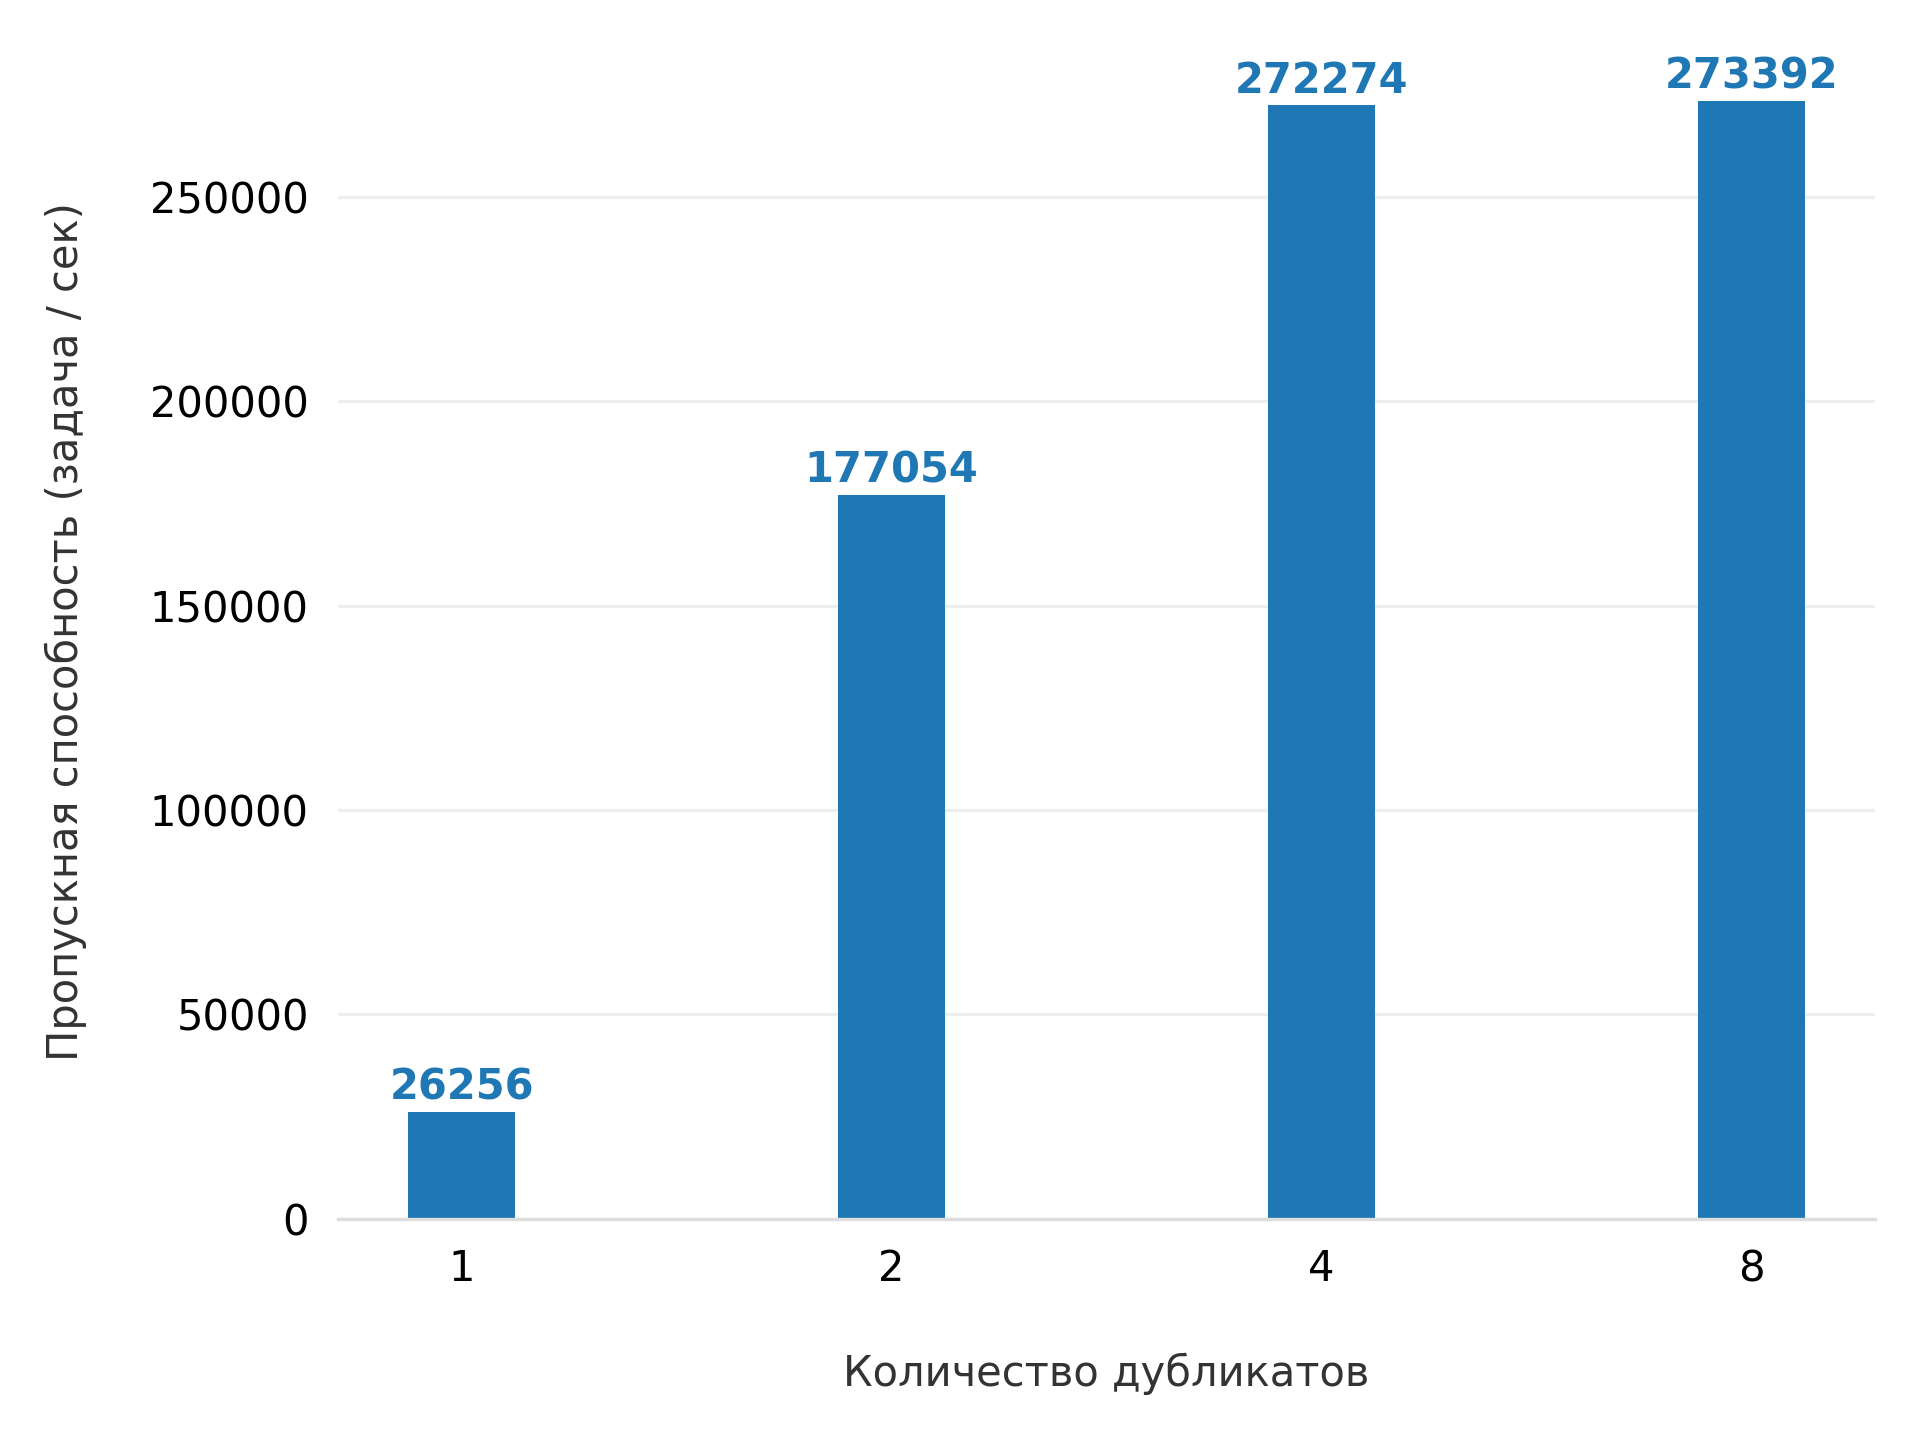
\includegraphics[scale=0.80]{pictures/rt_nsapwner128_nspawn1000.png}}
    \end{center}

    \caption{Производительность системы при использовании нескольких рантаймов}
    \label{fig:tatlin:multi_rt:eval}
\end{figure}

Из изображения заметным становится увеличение производительности при увеличении количества рантаймов.

\subsection{Вывод}

При локализации и изоляции меньших групп воркеров с отдельными глобальными очередями в рамках отдельных инстанцов рантаймов наблюдается увеличение пропускной способности. Это может происходить по многим причинам, некоторые из которых перечислены далее:

\begin{itemize}
    \item Меньшая борьба за глобальную очередь, за счет деления воркеров между несколькими очередями, что соответствует гипотезе инженеров из \verb|TATLIN.BACKUP|.
    \item Меньшее количество воркеров пытаются украсть задачи у соседей, из-за изоляции воркеров в различных инстансах рантама. Механизм кражи задач эксплуатирует lock free реализацию локальной очереди, что может приводить к нежелательным синхронзациям межу различными потоками и уменьшать пропускную способность.
\end{itemize}

Не зависимо от причин, использование нескольких рантаймов позволяет увеличить пропускную способность, а потому далее будет исследована возможность использования конструкции состоящей из нескольких рантаймов.
